\section{RRT  Class Reference}
\label{class_RRT}\index{RRT@{RRT}}
The base class, which generates a single Rapidly-exploring Random Tree. 


{\tt \#include $<$rrt.h$>$}

Inheritance diagram for RRT::\begin{figure}[H]
\begin{center}
\leavevmode
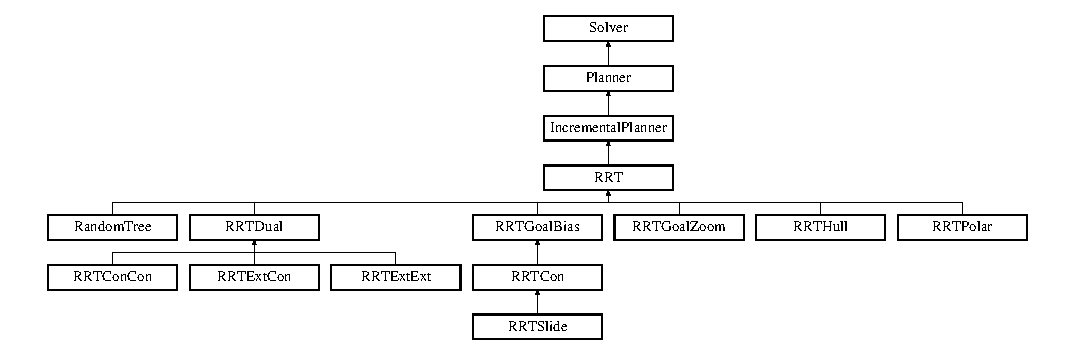
\includegraphics[height=4.34109cm]{class_RRT}
\end{center}
\end{figure}
\subsection*{Public Methods}
\begin{CompactItemize}
\item 
{\bf RRT} ({\bf Problem} $\ast$problem)
\begin{CompactList}\small\item\em A constructor that initializes data members.\item\end{CompactList}\item 
virtual {\bf $\sim$RRT} ()
\begin{CompactList}\small\item\em Empty destructor.\item\end{CompactList}\item 
virtual void {\bf Reset} ()
\begin{CompactList}\small\item\em Reset the planner.\item\end{CompactList}\item 
virtual bool {\bf Plan} ()
\begin{CompactList}\small\item\em Attempt to solve an Initial-Goal query by growing an RRT.\item\end{CompactList}\end{CompactItemize}
\subsection*{Public Attributes}
\begin{CompactItemize}
\item 
bool {\bf Use\-ANN}
\begin{CompactList}\small\item\em If true, then the ANN package is used for nearest neighbors. It assumes R$^\wedge$n topology and Euclidean metric. The default is false.\item\end{CompactList}\item 
double {\bf Goal\-Dist}
\begin{CompactList}\small\item\em The distance of the closest RRT {\bf MSLNode} {\rm (p.\,\pageref{class_MSLNode})} to the goal.\item\end{CompactList}\item 
{\bf MSLVector} {\bf Best\-State}
\begin{CompactList}\small\item\em The closest state to the goal so far (not used in dual-tree planners).\item\end{CompactList}\item 
double {\bf Connect\-Time\-Limit}
\begin{CompactList}\small\item\em The maximum amount of time to move in a Connect step (default = INFINITY).\item\end{CompactList}\item 
int {\bf Satisfied\-Count}
\begin{CompactList}\small\item\em Number of times the collision checker has been called.\item\end{CompactList}\end{CompactItemize}
\subsection*{Protected Methods}
\begin{CompactItemize}
\item 
virtual {\bf MSLVector} {\bf Select\-Input} (const {\bf MSLVector} \&x1, const {\bf MSLVector} \&x2, {\bf MSLVector} \&nx\_\-best, bool \&success, bool forward)
\begin{CompactList}\small\item\em Select the input that gets closest to x2 from x1.\item\end{CompactList}\item 
virtual {\bf MSLNode}$\ast$ {\bf Select\-Node} (const {\bf MSLVector} \&x, {\bf MSLTree} $\ast$t, bool forward)
\begin{CompactList}\small\item\em Return the nearest neighbor in the graph.\item\end{CompactList}\item 
virtual bool {\bf Extend} (const {\bf MSLVector} \&x, {\bf MSLTree} $\ast$t, {\bf MSLNode} $\ast$\&nn, bool forward)
\begin{CompactList}\small\item\em Incrementally extend the RRT.\item\end{CompactList}\item 
virtual bool {\bf Connect} (const {\bf MSLVector} \&x, {\bf MSLTree} $\ast$t, {\bf MSLNode} $\ast$\&nn, bool forward)
\begin{CompactList}\small\item\em Iterated Extend.\item\end{CompactList}\item 
virtual {\bf MSLVector} {\bf Choose\-State} ()
\begin{CompactList}\small\item\em Pick a state using some sampling technique.\item\end{CompactList}\end{CompactItemize}


\subsection{Detailed Description}
The base class, which generates a single Rapidly-exploring Random Tree.

The base class for the planners based on Rapidly-exploring  Random Trees. In the base class, a single tree is generated without any regard to the Goal\-State. The best planners to try are  {\bf RRTGoal\-Bias} {\rm (p.\,\pageref{class_RRTGoalBias})} and {\bf RRTGoal\-Zoom} {\rm (p.\,\pageref{class_RRTGoalZoom})} for single trees, and {\bf RRTCon\-Con} {\rm (p.\,\pageref{class_RRTConCon})} and  {\bf RRTExt\-Ext} {\rm (p.\,\pageref{class_RRTExtExt})} for dual trees. Dual tree approaches are much more efficient than single tree approaches, assuming dual trees can be applied. 



\subsection{Constructor \& Destructor Documentation}
\index{RRT@{RRT}!RRT@{RRT}}
\index{RRT@{RRT}!RRT@{RRT}}
\subsubsection{\setlength{\rightskip}{0pt plus 5cm}RRT::RRT ({\bf Problem} $\ast$ {\em problem})}\label{class_RRT_a0}


A constructor that initializes data members.

\index{RRT@{RRT}!~RRT@{$\sim$RRT}}
\index{~RRT@{$\sim$RRT}!RRT@{RRT}}
\subsubsection{\setlength{\rightskip}{0pt plus 5cm}RRT::$\sim$RRT ()\hspace{0.3cm}{\tt  [inline, virtual]}}\label{class_RRT_a1}


Empty destructor.



\subsection{Member Function Documentation}
\index{RRT@{RRT}!ChooseState@{ChooseState}}
\index{ChooseState@{ChooseState}!RRT@{RRT}}
\subsubsection{\setlength{\rightskip}{0pt plus 5cm}{\bf MSLVector} RRT::Choose\-State ()\hspace{0.3cm}{\tt  [protected, virtual]}}\label{class_RRT_b4}


Pick a state using some sampling technique.



Reimplemented in {\bf RRTGoal\-Bias} {\rm (p.\,\pageref{class_RRTGoalBias_b0})}, {\bf RRTGoal\-Zoom} {\rm (p.\,\pageref{class_RRTGoalZoom_b0})}, {\bf RRTPolar} {\rm (p.\,\pageref{class_RRTPolar_b0})}, and {\bf RRTHull} {\rm (p.\,\pageref{class_RRTHull_b0})}.\index{RRT@{RRT}!Connect@{Connect}}
\index{Connect@{Connect}!RRT@{RRT}}
\subsubsection{\setlength{\rightskip}{0pt plus 5cm}bool RRT::Connect (const {\bf MSLVector} \& {\em x}, {\bf MSLTree} $\ast$ {\em t}, {\bf MSLNode} $\ast$\& {\em nn}, bool {\em forward})\hspace{0.3cm}{\tt  [protected, virtual]}}\label{class_RRT_b3}


Iterated Extend.



Reimplemented in {\bf RRTSlide} {\rm (p.\,\pageref{class_RRTSlide_a3})}.\index{RRT@{RRT}!Extend@{Extend}}
\index{Extend@{Extend}!RRT@{RRT}}
\subsubsection{\setlength{\rightskip}{0pt plus 5cm}bool RRT::Extend (const {\bf MSLVector} \& {\em x}, {\bf MSLTree} $\ast$ {\em t}, {\bf MSLNode} $\ast$\& {\em nn}, bool {\em forward})\hspace{0.3cm}{\tt  [protected, virtual]}}\label{class_RRT_b2}


Incrementally extend the RRT.

\index{RRT@{RRT}!Plan@{Plan}}
\index{Plan@{Plan}!RRT@{RRT}}
\subsubsection{\setlength{\rightskip}{0pt plus 5cm}bool RRT::Plan ()\hspace{0.3cm}{\tt  [virtual]}}\label{class_RRT_a3}


Attempt to solve an Initial-Goal query by growing an RRT.



Reimplemented from {\bf Planner} {\rm (p.\,\pageref{class_Planner_a4})}.

Reimplemented in {\bf RRTCon} {\rm (p.\,\pageref{class_RRTCon_a2})}, {\bf RRTDual} {\rm (p.\,\pageref{class_RRTDual_a2})}, {\bf RRTExt\-Ext} {\rm (p.\,\pageref{class_RRTExtExt_a2})}, {\bf RRTExt\-Con} {\rm (p.\,\pageref{class_RRTExtCon_a2})}, and {\bf RRTCon\-Con} {\rm (p.\,\pageref{class_RRTConCon_a2})}.\index{RRT@{RRT}!Reset@{Reset}}
\index{Reset@{Reset}!RRT@{RRT}}
\subsubsection{\setlength{\rightskip}{0pt plus 5cm}void RRT::Reset ()\hspace{0.3cm}{\tt  [virtual]}}\label{class_RRT_a2}


Reset the planner.



Reimplemented from {\bf Planner} {\rm (p.\,\pageref{class_Planner_a2})}.\index{RRT@{RRT}!SelectInput@{SelectInput}}
\index{SelectInput@{SelectInput}!RRT@{RRT}}
\subsubsection{\setlength{\rightskip}{0pt plus 5cm}{\bf MSLVector} RRT::Select\-Input (const {\bf MSLVector} \& {\em x1}, const {\bf MSLVector} \& {\em x2}, {\bf MSLVector} \& {\em nx\_\-best}, bool \& {\em success}, bool {\em forward})\hspace{0.3cm}{\tt  [protected, virtual]}}\label{class_RRT_b0}


Select the input that gets closest to x2 from x1.



Reimplemented in {\bf Random\-Tree} {\rm (p.\,\pageref{class_RandomTree_b1})}, and {\bf RRTSlide} {\rm (p.\,\pageref{class_RRTSlide_a2})}.\index{RRT@{RRT}!SelectNode@{SelectNode}}
\index{SelectNode@{SelectNode}!RRT@{RRT}}
\subsubsection{\setlength{\rightskip}{0pt plus 5cm}{\bf MSLNode} $\ast$ RRT::Select\-Node (const {\bf MSLVector} \& {\em x}, {\bf MSLTree} $\ast$ {\em t}, bool {\em forward})\hspace{0.3cm}{\tt  [protected, virtual]}}\label{class_RRT_b1}


Return the nearest neighbor in the graph.



Reimplemented in {\bf Random\-Tree} {\rm (p.\,\pageref{class_RandomTree_b0})}.

\subsection{Member Data Documentation}
\index{RRT@{RRT}!BestState@{BestState}}
\index{BestState@{BestState}!RRT@{RRT}}
\subsubsection{\setlength{\rightskip}{0pt plus 5cm}{\bf MSLVector} RRT::Best\-State}\label{class_RRT_m2}


The closest state to the goal so far (not used in dual-tree planners).

\index{RRT@{RRT}!ConnectTimeLimit@{ConnectTimeLimit}}
\index{ConnectTimeLimit@{ConnectTimeLimit}!RRT@{RRT}}
\subsubsection{\setlength{\rightskip}{0pt plus 5cm}double RRT::Connect\-Time\-Limit}\label{class_RRT_m3}


The maximum amount of time to move in a Connect step (default = INFINITY).

\index{RRT@{RRT}!GoalDist@{GoalDist}}
\index{GoalDist@{GoalDist}!RRT@{RRT}}
\subsubsection{\setlength{\rightskip}{0pt plus 5cm}double RRT::Goal\-Dist}\label{class_RRT_m1}


The distance of the closest RRT {\bf MSLNode} {\rm (p.\,\pageref{class_MSLNode})} to the goal.

\index{RRT@{RRT}!SatisfiedCount@{SatisfiedCount}}
\index{SatisfiedCount@{SatisfiedCount}!RRT@{RRT}}
\subsubsection{\setlength{\rightskip}{0pt plus 5cm}int RRT::Satisfied\-Count}\label{class_RRT_m4}


Number of times the collision checker has been called.

\index{RRT@{RRT}!UseANN@{UseANN}}
\index{UseANN@{UseANN}!RRT@{RRT}}
\subsubsection{\setlength{\rightskip}{0pt plus 5cm}bool RRT::Use\-ANN}\label{class_RRT_m0}


If true, then the ANN package is used for nearest neighbors. It assumes R$^\wedge$n topology and Euclidean metric. The default is false.



The documentation for this class was generated from the following file:\begin{CompactItemize}
\item 
{\bf rrt.h}\end{CompactItemize}
